\chapter{History of cross-platform development}
\label{chap:ch1}

\indent
\par



%\begin{figure}[htbp]
	%\centering
	%	\includegraphics[scale=0.65]{./figures/fig_3_1.eps}
	%\caption{Ciclul de dezvoltare al sistemelor bazate pe componente adaptat modelului cascadã}
	%\label{FigCBSD}
%\end{figure}
In this chapter, I will elaborate on the progresses made throughout the decades regarding designing software and the evolution of hardware, and see how we ended up with cross-platform development as a necessity.

\section{The 1940-1970 timeline}

\subsection{The 1940's}

\par

During this decade, the "Big Bang" happened.
John Mauchly and Presper Eckert, designed and built the "first digital, electronic computer"\cite{eniacHistory} and came up with the legendary ENIAC.
A computer that was designed with a military goal in mind.
ENIAC was developed at the University of Pennsylvania, being funded by the U.S.
Army, mainly because the teams at the other Universities were not able to keep up with the Army's needs for computing artillery firing tables "for the war 
effort".\cite{eniacDesign}

\par
This computer revolutionized computations as it was the first machine to ever allow any kind of stored procedures, by introducing plugboard wiring and portable function tables in favor of the previous punch cards.
Plugboards were connecting switches, which were "capable of storing one complex instruction for the use of the accumulator".\cite{eniacSwitches}
This meant that, the entirety of the computation was digital, and reconfigurable.
Unfortunately, it also meant that, between each run or change, the computer had to be shut down so the wiring could be redone.
\begin{figure}[htbp]
    \centering
    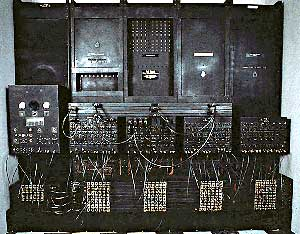
\includegraphics[scale=0.5]{pictures/ENIAC_plugboard_switches.jpg}
    \caption{ENIAC plugboards and switches}
    \label{eniacPlugboardSwitches}
\end{figure}
\par
But, even so, a good algorithm structure was needed, that being mainly because 'these architectural differences lead to some differences in the approach needed for programming'\cite{eniacDesign}.
So the operators of the machine came upon some design and operation principles, that are still observable in the modern world, such as 'Dataflow', 'Parallelism' and 'Looping and branching' \cite{eniacDesign}


\subsection{The 1950's}
\par
Software engineering and designing became a subject of discussion as early as the 1950's.
During those days, this terminology meant something entirely different than what we know of today.
The quote that depicted it quite accurate is: `\textit{Software engineering is like hardware engineering}`\cite{boehmb06}.
This is mainly because software was regarded as building a machine: you embody a plan, manually check it and then get it running on the computer.
\par
The biggest invention of this decade was the concept of storing, organizing and manipulating data.
It is during these times that it got a name, "data processing"\cite{firstDBMS}.
It is also now when the storage, retrieval, and updating of data has been a "key requirement for most computer applications"\cite{firstDBMS}.
These are things that followed up and evolved into the modern world, and they can be observable as most up-to-date applications require enormous data volumes.
Data started to play an important role.
It was regarded as one of the building blocks of applications back then.
This is also another pattern that is kept into the modern development world.
\par
In this same decade, more specifically in 1952, the first compiler was made, for the A-0 system.
This compiler was introduced and put into practice by one of the founding figures of the programming field, that being Grace Hopper.
This represented a turning point, as she proved that computers should understand "human-like" languages\cite{a0compiler}, not the other way around.
Now the tool of software became a much more teachable subject, and had the potential of turning to be more at-hand for everybody.
In 1953 she developed A-2, which is considered to be the first open-source piece of software ever.
That is due to the fact that its source code was given to the customers and they were encouraged to send in possible improvements.


\par
The first commercially-available compiler was put on the market not that later on.
It is the FORTRAN, "formula translator"\cite{a0compiler}, compiler that was developed by IBM in 1957, for the 704 computer.
It is now that we can see a mould for software.
During the same decade, the first pieces of both open-source and closed-source software were developed and put on the market.



\subsection{The 1960's}
During this time period, the machines got a bit more user friendly and code became easily replaceable.
This turned software into something far different to hardware.
COBOL is now introduced to the market, and it made a case for itself.
It is the first programming language that was considered easy to use and read, and that introduced the concept of machine abstraction.
This meant that it did not require a dedicated machine to run.
It was, in a very abstract and distant way, the first piece of cross-platform software.

\par
Now, the ability to rewrite code enabled developers to turn towards a "code and fix" approach\cite{boehmb06}.
This meant that coding was something that did not require as much manual calculations, and that can be thought of and corrected along the way.
Not only that, but it is the first time during this decade that a problem was eradicated: having exact hardware in order to collaborate on development.
This is considered to be a menial job for the modern programmers, but during those times it was a long due issue.
\par
This is one of the biggest turning points in software design, as it allowed for a practice that is still put to good use today.
Correction of code, be it from a logical or opinionated point of view, during development lead to branching and forking, tools that are still used in modern development.



\section{The 1970 - 1990 timeline}
\subsection{The 1970's}
This decade is perhaps the most important step in software development.
This is the decade that made modern computing the thing that we know and love.
In 1972, Dennis M.
Ritchie and his team created the C programming language.
To say it was revolutionary, was an understatement.
This project turned Dennis Ritchie into a titan and unforgettable figure of the software world.
He was a "bearded, somewhat disheveled computer scientist"\cite{ritchieJobs} that stays at the foundation of the things we make most use of today, for exmaple the internet.

\begin{figure}[htbp]
    \centering
    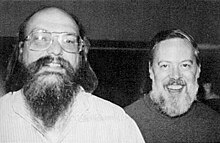
\includegraphics[scale=0.7]{pictures/KenThompson_and_DennisRitchie1973.jpg}
    \caption{Ken Thompson and Dennis Ritchie, 1973}
    \label{unixMakers}
\end{figure}

\par
C is a language that derived from BCPL (Basic Combined Programming Language).
It became relevant when, yet again, Dennis Ritchie decided to use it in order to re-write the source code of the UNIX operating system.
Such and operation was deemed necessary by him mainly because the U.S government categorized the capitalism of such a product as a violation the "Sherman Antitrust Act"\cite{unixRepo}.
Due to this, AT\&T released the Operating System as royalty-free, but later however licenses became a bigger obstruction, hence the limitations in the access of the source code.
Then Dennis Ritchie decided to re-write the whole OS in the high-level programming language in C, in 1973.
This project, although later forked into many other operating systems such MacOS or GNU/Linux, was maintained and developed up to this day to the FreeBSD project.
A part of the legacy assembly source code of UNIX is still on GitHub, at the repository 'dspinellis/unix-history-make'.

\begin{figure}[htbp]
    \centering
    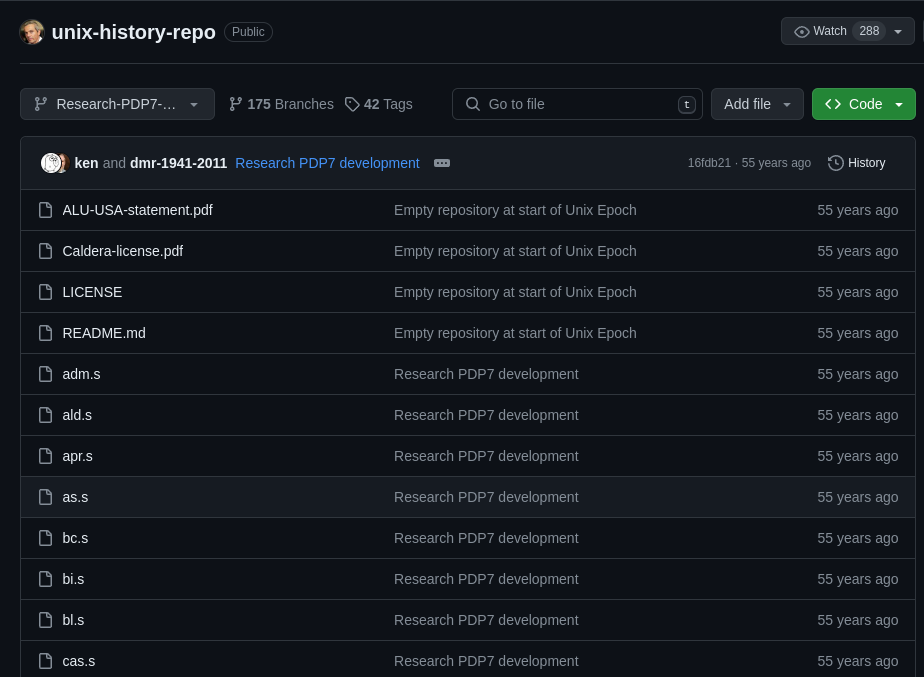
\includegraphics[scale=0.5]{pictures/unix_repo.png}
    \caption{TODO:change to white theme Repository containing the assembly source code of UNIX}
    \label{unixRepo}
\end{figure}


\subsection{The 1980's}
During the 80's, software design became an area on interest for most people involved in the computer science field.
One of the earliest approaches of software design is the Layered architecture.
This was firstly introduced as a need because of the way computer networks were operating.
Now, files were getting bigger and because of that, "The programmer must maintain descriptions of
how various alternative designs are distributed among files"\cite{layeredArchitecure80s}.

\par
Along with these software design paradigms, this decade introduced the first implementation of a version control system.
It worked quite similarly to the modern approaches.
It stored the differentials of the files in a 'delta' file\cite{layeredArchitecure80s}.
This file was one of the deterministic factors for which version control and layered architecture were introduced.
As files grew bigger in size, the delta file associated with it was also getting clunkier, thus making reverting or alternating changes a time and memory-consuming task, and by separating the files into smaller ones, each depending on the other one, this process would be optimized.

\par
This decade brings the most enhancing and used tool of the modern world, the internet.
Although it is believed that invented rather earlier, in the late 60's, it is in 1983 when ARPANET and DDN (Defense Data Network) switched to the TCP/IP standard, "so that computers of many kinds could communicate with each other, no matter what kind of network they were connected to in the Internet".\cite{arpanetDdn} This was a big leap, as ARPANET was an already enormous cluster of interconnected computers, therefore the computers entering the network would have access to them.

\begin{figure}[htbp]
    \centering
    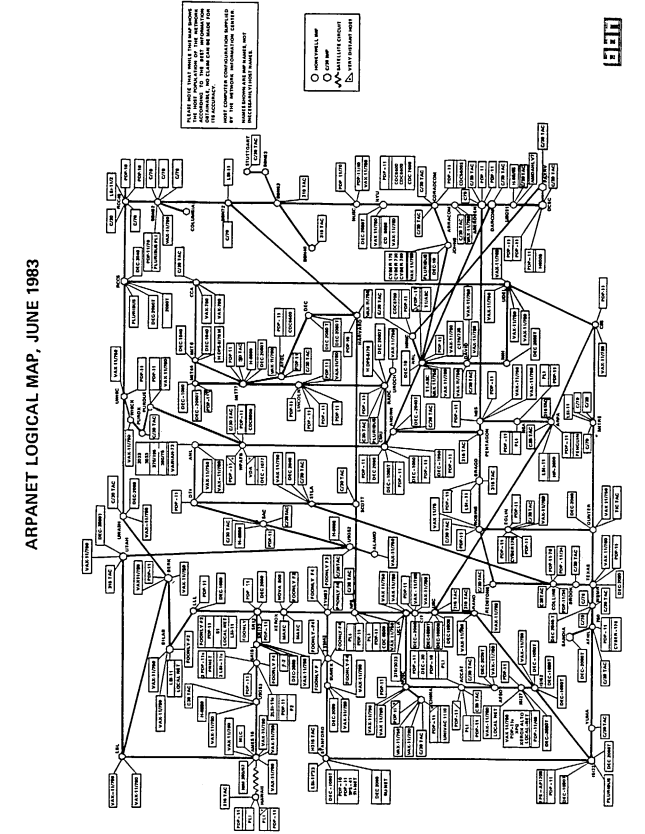
\includegraphics[angle=270,scale=0.35]{pictures/arpanet.png}
    \caption{ARPANET logical map, 1983}
    \label{arpanetLogicaMap}
\end{figure}


\par
Due to this, a doubling of household computers happened until the 90's.
This meant that more people were put on the network, and, due to this, all the computer owners had access to each other's data and information, should they wanted to access it.

\begin{center}
    \begin{tabular}{|| c | c ||}
          \hline
          \textbf{Year} & \textbf{Percentage} \\
          \hline
          1980 & 2.8\% \\
          \hline
          1982 & 6.2\% \\
          \hline
          1983 & 7.3\% \\
          \hline
          1984 & 8.4\% \\
          \hline
          1986 & 9.5\% \\
          \hline
          1988 & 12.5\% \\
          \hline
          1989 & 15.0\% \\
          \hline
    \end{tabular}
\end{center}

\par
As you can see, the biggest jump in the percentages happened between 1980 and 1982.
But, since ARPANET switched their protocols in 1983, the number of computers in personal households has grown by a staggering 7.7\%, a bit more than double.



\subsection{The 1990's}
This decade has been the most influential one for the modern world, and especially for the computing area.
With the evergrowing increase in computer-owning households and the creation of the internet, we see how this affected the development process, thus leading to a series of projects that are major key-factors in our current timeline.

\par
In 1990, we see the first true creation of cross-platform software.
At CERN, Switzerland, Tim Berners-Lee submits two ideas for what should be the Web, back in March 1989.
Until the Christmas of 1990, he contoured the World Wide Web, making the first prototype for it.
The intention of this project was to be "a pool of human knowledge", thus allowing for ease of communication between people who were geologically disjointed\cite{worldWideWeb}.

\par
This project offered features that are still generally available today, such as a server, HTML, the first web programming language, URL's and the first browser.

\section{The 2000's}
\subsection{First definition}
Now, during this decade we can see some of the first mentions of the term "cross-platform development".
That is due to the fact that more and more "platforms" (example: Windows, MacOS) started rising and gaining popularity, and certain large applications needed to behave and act accordingly on all of them.
I will refer to "platform" from now on as development environments, for example Android meaning not only the mobile phone operating system, but also the ecosystem surrounding it, such as smartwatches or TV's.


\par
Some of the first people that proposed this terminology were Bishop J.
and Horspool N., who also gave the first definition to this development branch.
They described the product of it as "software that exists in different versions so that it is available on more than one platform"\cite{firstDefinition}, all the way back in 2006.
In this definition, their meaning of platform is the same as the one I mentioned earlier, because back then the definition was a bit more general, such as "language, operating system, computer, or some combination".
In the same time-period, the Web was starting a world-conquering journey.
Along with it, it brought a whole toolkit of development principles and design patterns, with component-based development being the most praised one.
This is also mentioned and observed by the aforementioned authors, whom agree that component-based development  has made a good impact  toward satisfying "both parts of the definition."\cite{firstDefinition}
\subsection{First toolkits}
The idea of cross-platform development was initially brought as a fix for one of the bigger issues developers faced at the time, and that is building graphical user interfaces (GUI's).
This in itself represented a dilemma because for every platform there were dedicated tools and specific programming languages, for example for Windows there was exclusively .NET with the C\# programming language.
This inherently meant that there was no uniform way of developing such GUI's across platforms.
There is also acknowledgement in this, starting with the earliest days.
Due to such history, there came the stigma that cross-platform toolkits are "integral to GUI development"\cite{firstDefinition}.

\par
Because of this, we can also observe the rise in popularity of some toolkits that were not very seriously taken considered before this realization, such as Qt or GTK+.
These are some of the first cross-platform frameworks that are still used today at a production level, and we can see them used in many well-known applications, such as Spotify for Qt, or the GNOME desktop environment for GTK+.
They are trying to achieve different goals, but one thing that they have in common is that both Qt and GTK+ define a collection of widgets that should work as "platform independent"\cite{firstDefinition}.
This then allowed for the developers to apply a "learn once, code everywhere" approach.
